\section{Results}
The first part of this project was to develop a model that classifies if a fish is present in a image. 
Using the default configurations in PyTorch this was acheived in short time.
The second part was to develop a model that could identify the kind of fish or if there was no fish. 
This proved to be much more challenging. In this section, the results of these models are discussed.


\begin{table}[h]
    \centering
    \begin{tabular}{lcccc}
        \hline
        & Accuracy & F1 Score & Precision & Recall \\
        \hline
        Res18 & 0.989 & 0.988 & 0.988 & 0.989 \\
        \hline
    \end{tabular}
    \caption{Binary Model performance metrics.}
    \label{tab:binarymetrics}
\end{table}


\begin{table}[h]
    \centering
    \begin{tabular}{lcccc}
        \hline
        & Accuracy & F1 Score & Precision & Recall \\
        \hline
        Res18 & 0.6928 & 0.7001 & 0.76663 & 0.87668 \\
        Res18 (Transfer Learning) & 0.989 & 0.988 & 0.988 & 0.989 \\
        Res50 & 0.989 & 0.988 & 0.988 & 0.989 \\
        Res50 (Transfer Learning) & 0.989 & 0.988 & 0.988 & 0.989 \\
        DenseNet & 0.989 & 0.988 & 0.988 & 0.989 \\
        DenseNet (Transfer Learning) & 0.989 & 0.988 & 0.988 & 0.989 \\
        RegNet & 0.989 & 0.988 & 0.988 & 0.989 \\
        RegNet (Transfer Learning) & 0.989 & 0.988 & 0.988 & 0.989 \\
        \hline
    \end{tabular}
    \caption{Multi Fish Model performance metrics.}
    \label{tab:multimetrics}
\end{table}


\subsection{Binary Res18 Model}
The first model ran was the binary classification case. A Res18 model was trained using transfer learning and the default PyTorch transforms. 
The default transforms are a Tesnor Conversion, a image resize to 256x256, a center crop, a float32 conversion, and a channel normalization.
Below is a representation of the transforms used in python


\begin{lstlisting}[language=python]
transform = T.Compose([
    T.Resize(256),
    T.CenterCrop(224),
    T.ToTensor(),
    T.Normalize(mean=[0.485, 0.456, 0.406],
                std=[0.229, 0.224, 0.225]),
])
\end{lstlisting}

The Res18 model performed very well with the default configurations. Table \ref{tab:binarymetrics} has the results for the performance of the model.
The confusion matrix, ROC graph, and loss graph can be seen at \ref{fig:binaryconf} \ref{fig:binaryroc} \ref{fig:binaryloss} respectively.
Achieving a 98\% accuracy was a very strong performance. This lead me to immediatetly attempting the multi fish problem.


\begin{figure}[htpb]
\centering
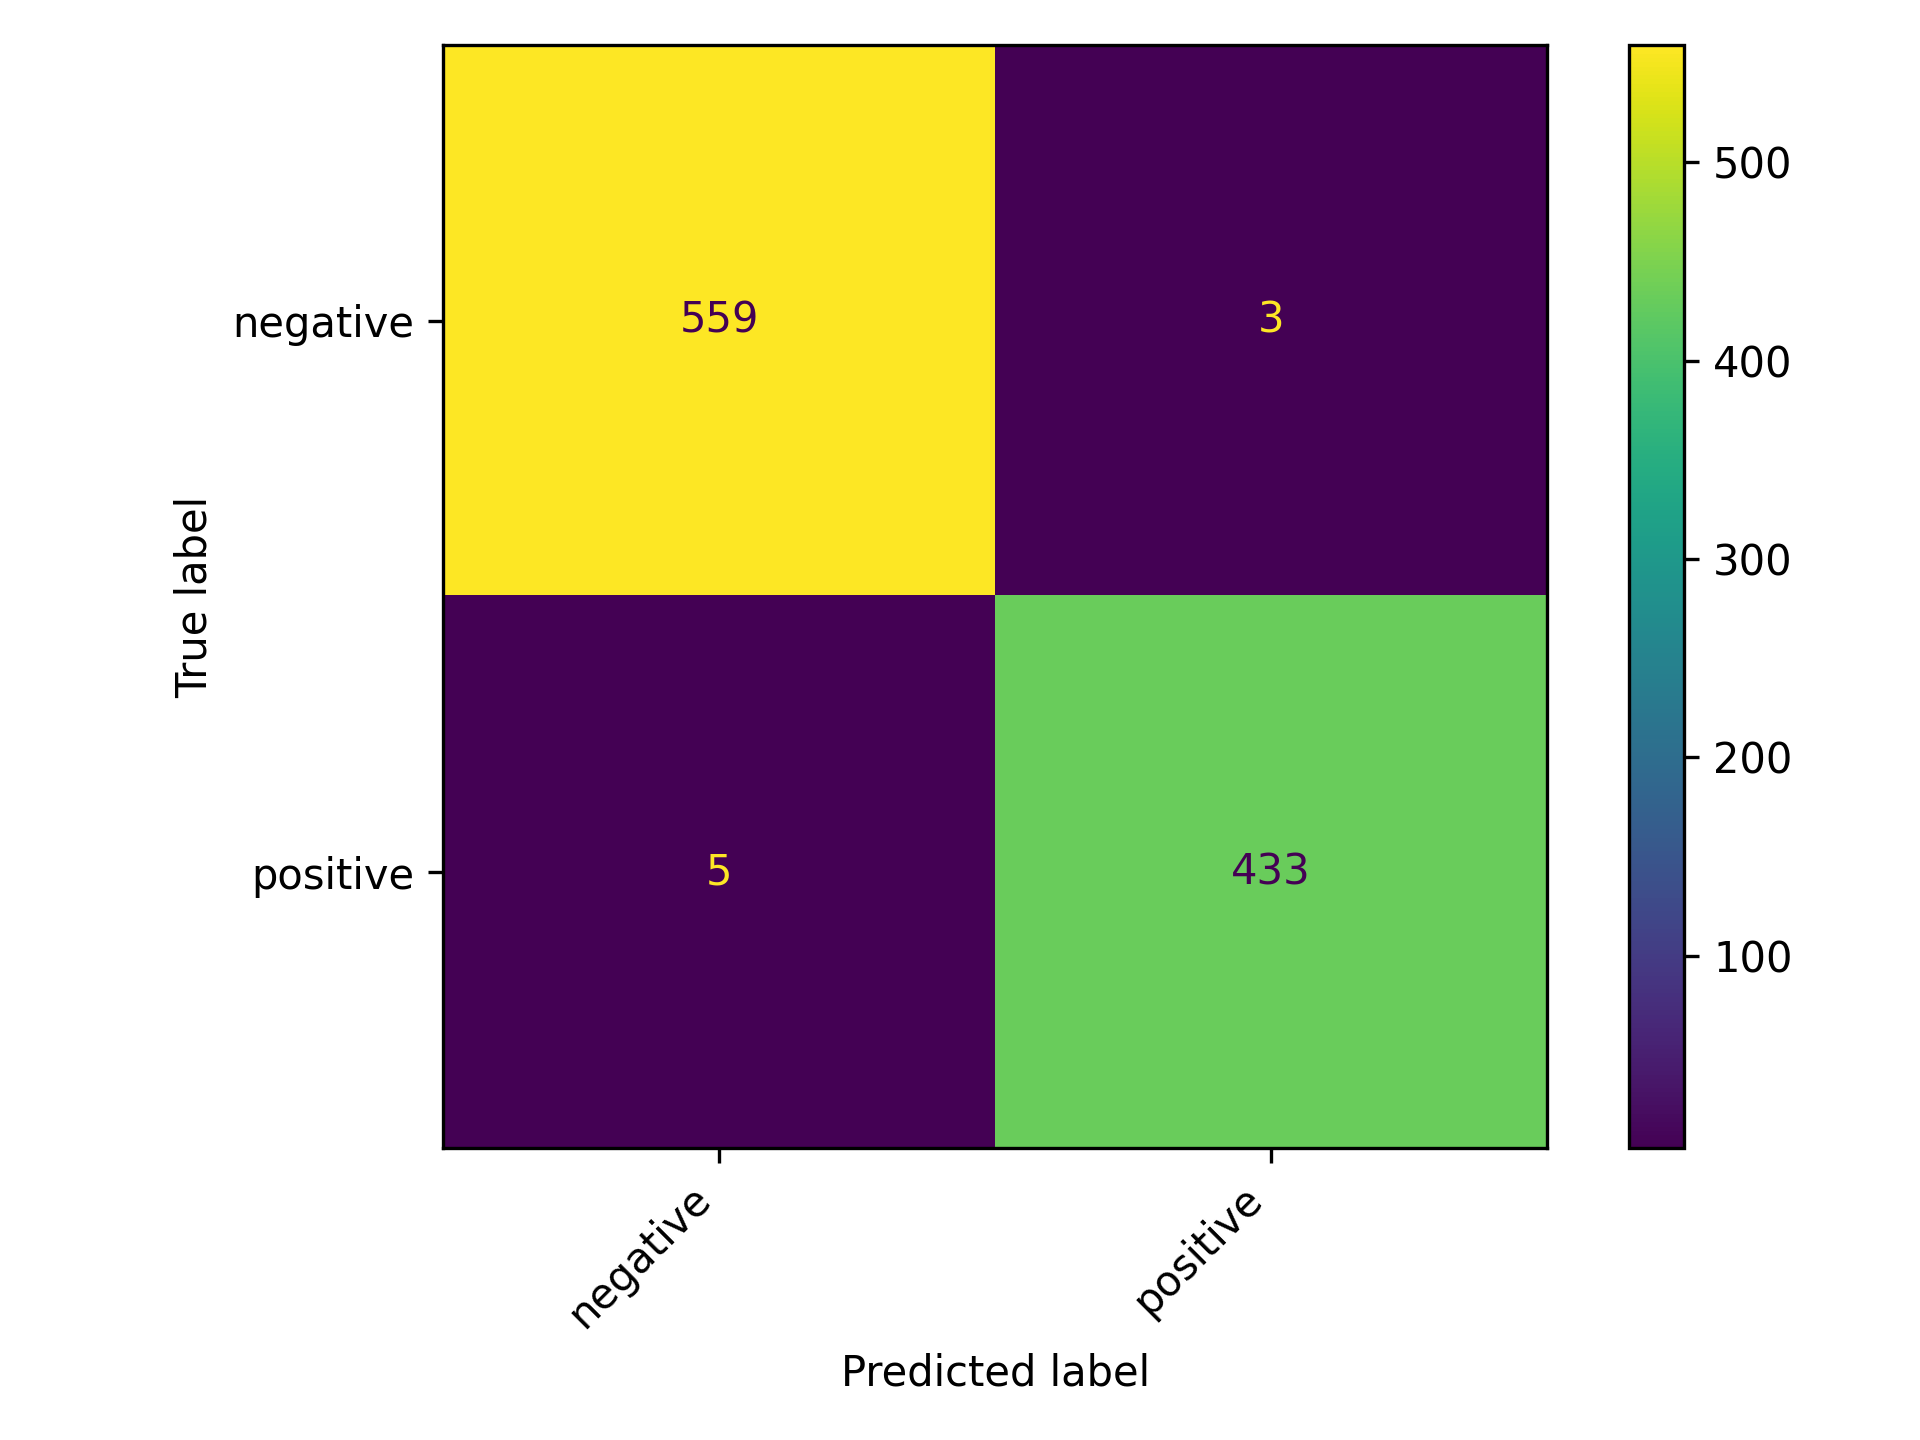
\includegraphics[width=0.8\linewidth]{../results/confusion/binary_weights_cm_2026-05-08_14-42.png}
    \caption{Confusion Matrix for the Res18 model trained on to predict the pressense of a Fish or No Fish.}
\label{fig:binaryconf}
\end{figure}

\begin{figure}[htpb]
\centering
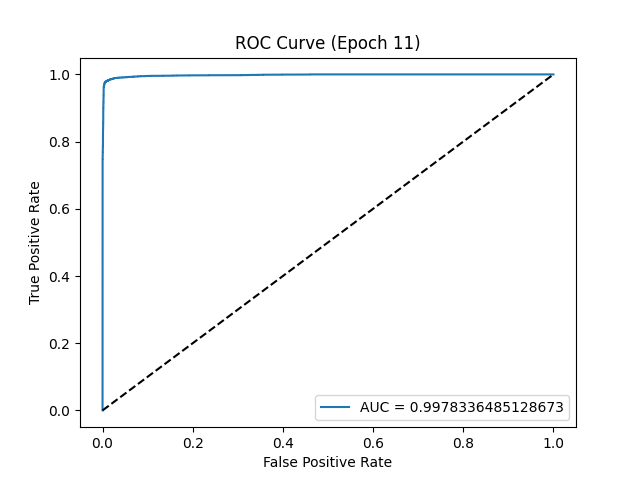
\includegraphics[width=0.8\linewidth]{../results/binary_weights_roc_2026-05-08_14-42.png}
    \caption{ROC for the Res18 model trained on to predict the pressense of a Fish or No Fish.}
\label{fig:binaryroc}
\end{figure}

\begin{figure}[htpb]
\centering
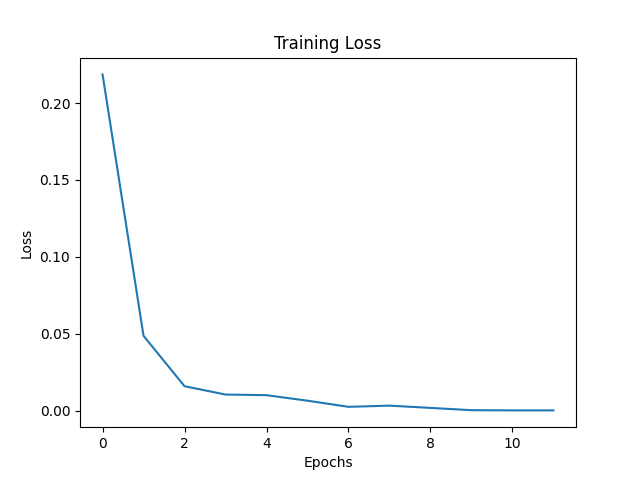
\includegraphics[width=0.8\linewidth]{../results/loss/binary_weights_loss_2026-05-08_14-42.png}
    \caption{Loss Graph for the Res18 model trained on to predict the pressense of a Fish or No Fish.}
\label{fig:binaryloss}
\end{figure}

\subsection{Res18 Multi Fish Model}
The Res18 model was used as the first model to attempt the multi fish classification problem. It was trained with and without transfer learning.
Utlizing transfer learning dramatically imrproved the prediction accuracy.




